The neutrinos in \nuprism are simulated with the T2K flux simulation tool called JNUBEAM.  The version of JNUBEAM used is consistent with what is currently used by T2K and it includes the modeling of hadronic interactions based on data from the NA61/SHINE experiment.  We define the off-axis angle for a particular neutrino as the angle between 
the beam axis and the vector from the average neutrino production point along the beam axis to the point
at which the neutrino crosses the flux plane, as illustrated in Fig.~\ref{fig:oa_def}.  The off-axis angle
is defined in terms of the average neutrino production point so that an off-axis angle observable can be
constructed based on the location of the interaction vertex in \nuprism.  The off-axis angle and energy 
dependence for each neutrino flavor is shown in Fig.~\ref{fig:sim_oa_enu}.  The neutrino flux files are produced
for both neutrino mode (focussing positively charged hadrons) and antineutrino mode (focussing negatively 
charged hadrons), although only the neutrino mode flux is used for the analysis presented in this note. 

\begin {figure}[htp]
  \begin{center}
    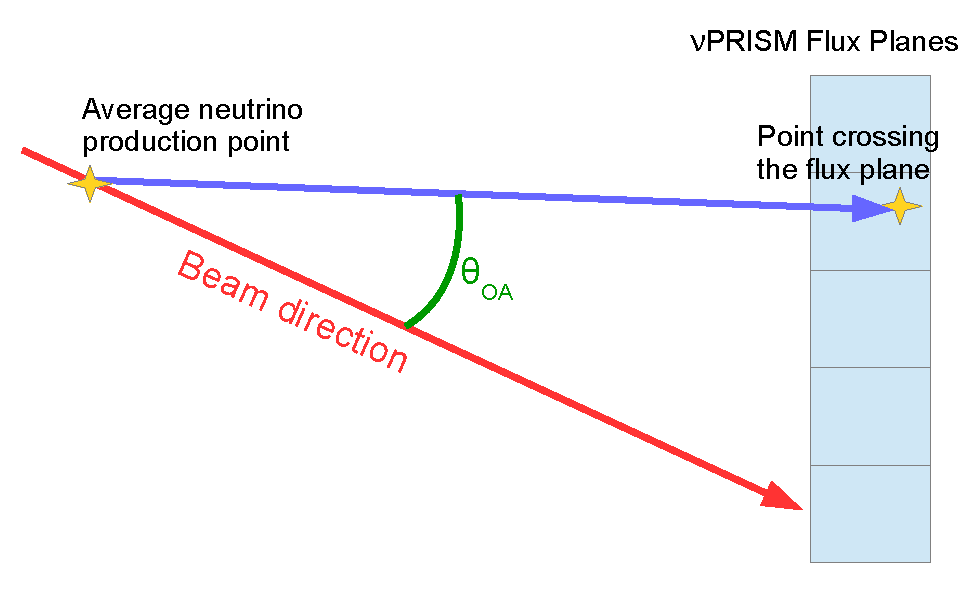
\includegraphics[width=0.45\textwidth]{figures/oa_definition.pdf}
    \caption{The definition of the off-axis angle for individual neutrinos.}
    \label{fig:oa_def}
  \end{center}
\end {figure}     

\begin {figure*}[htp]
  \begin{center}
    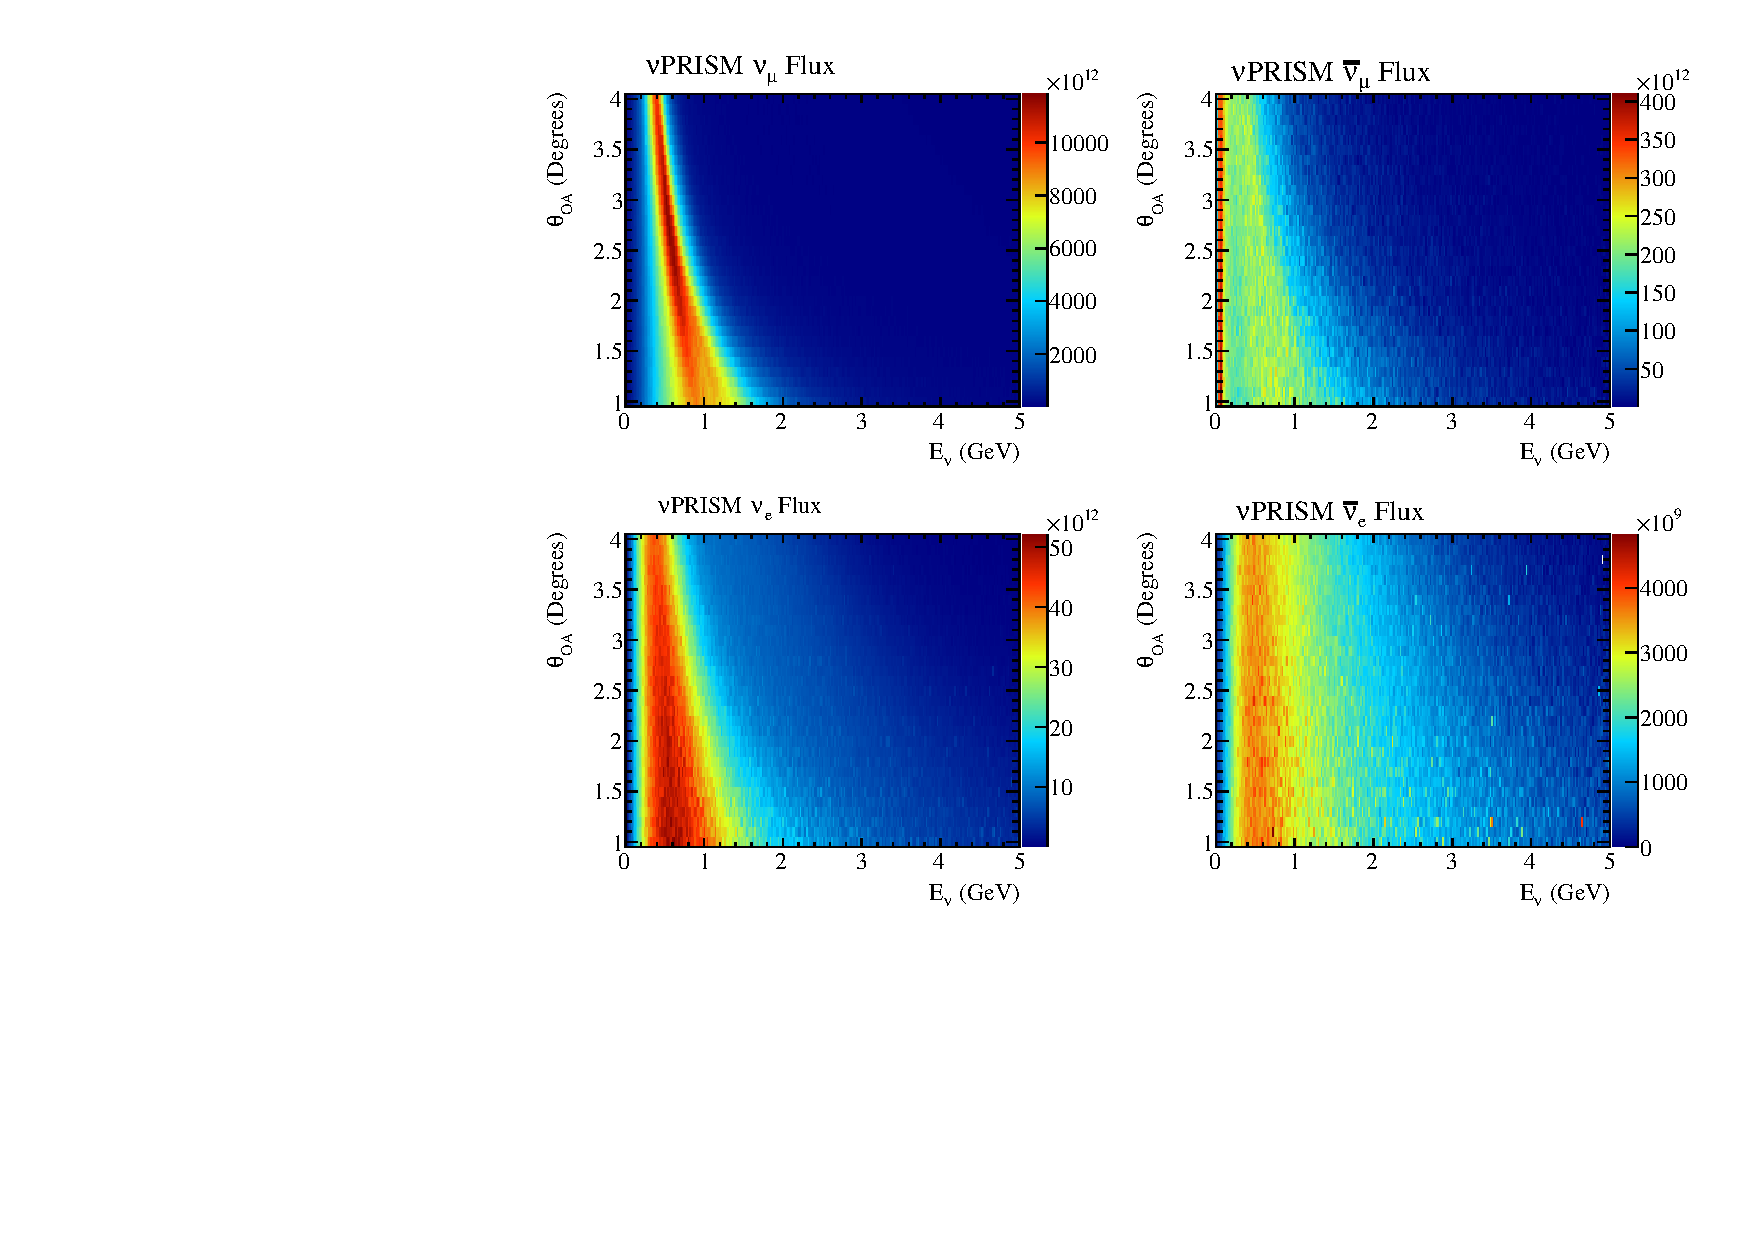
\includegraphics[width=0.9\textwidth]{figures/nuprism_oa_enu.pdf}
    \caption{The neutrino flux (arbitrary normalization) as a function of off-axis angle and energy
for each neutrino flavor with the horn in neutrino-mode operation.}
    \label{fig:sim_oa_enu}
  \end{center}
\end {figure*}  

%The neutrino interactions in the \nuprism water volume are modeled using NEUT 5.1.4.2.  The neutgeom package
%used for ND280 neutrino vector production has been adapted to handle arbitrary geometries. By adapting this package,
%we are able to generate vectors in the detector volume while accounting for the flux dependence on off-axis angle.
%A simple water column
%geometry was produced for \nuprism and interactions were generated using the previously described flux.  Interactions
%for the equivalent of 3.6e21 POT have been generated for neutrino mode operation, while a smaller sample equivalent to
%6.5e20 POT has been generated for antineutrino mode operation.  Interactions are also generated with NEUT 5.3.2 and the
%multinucleon events are skimmed and used for studies.  

The positions of the neutrino interaction vertices in the \nuprism water volume are shown in Fig.~\ref{fig:nu_vertex}.
The rate of simulated interactions has been cross checked against the observed INGRID rates% in Section~\ref{sec:nuprism_pileup}
and found to be consistent.

\begin {figure}[htp]
  \begin{center}
    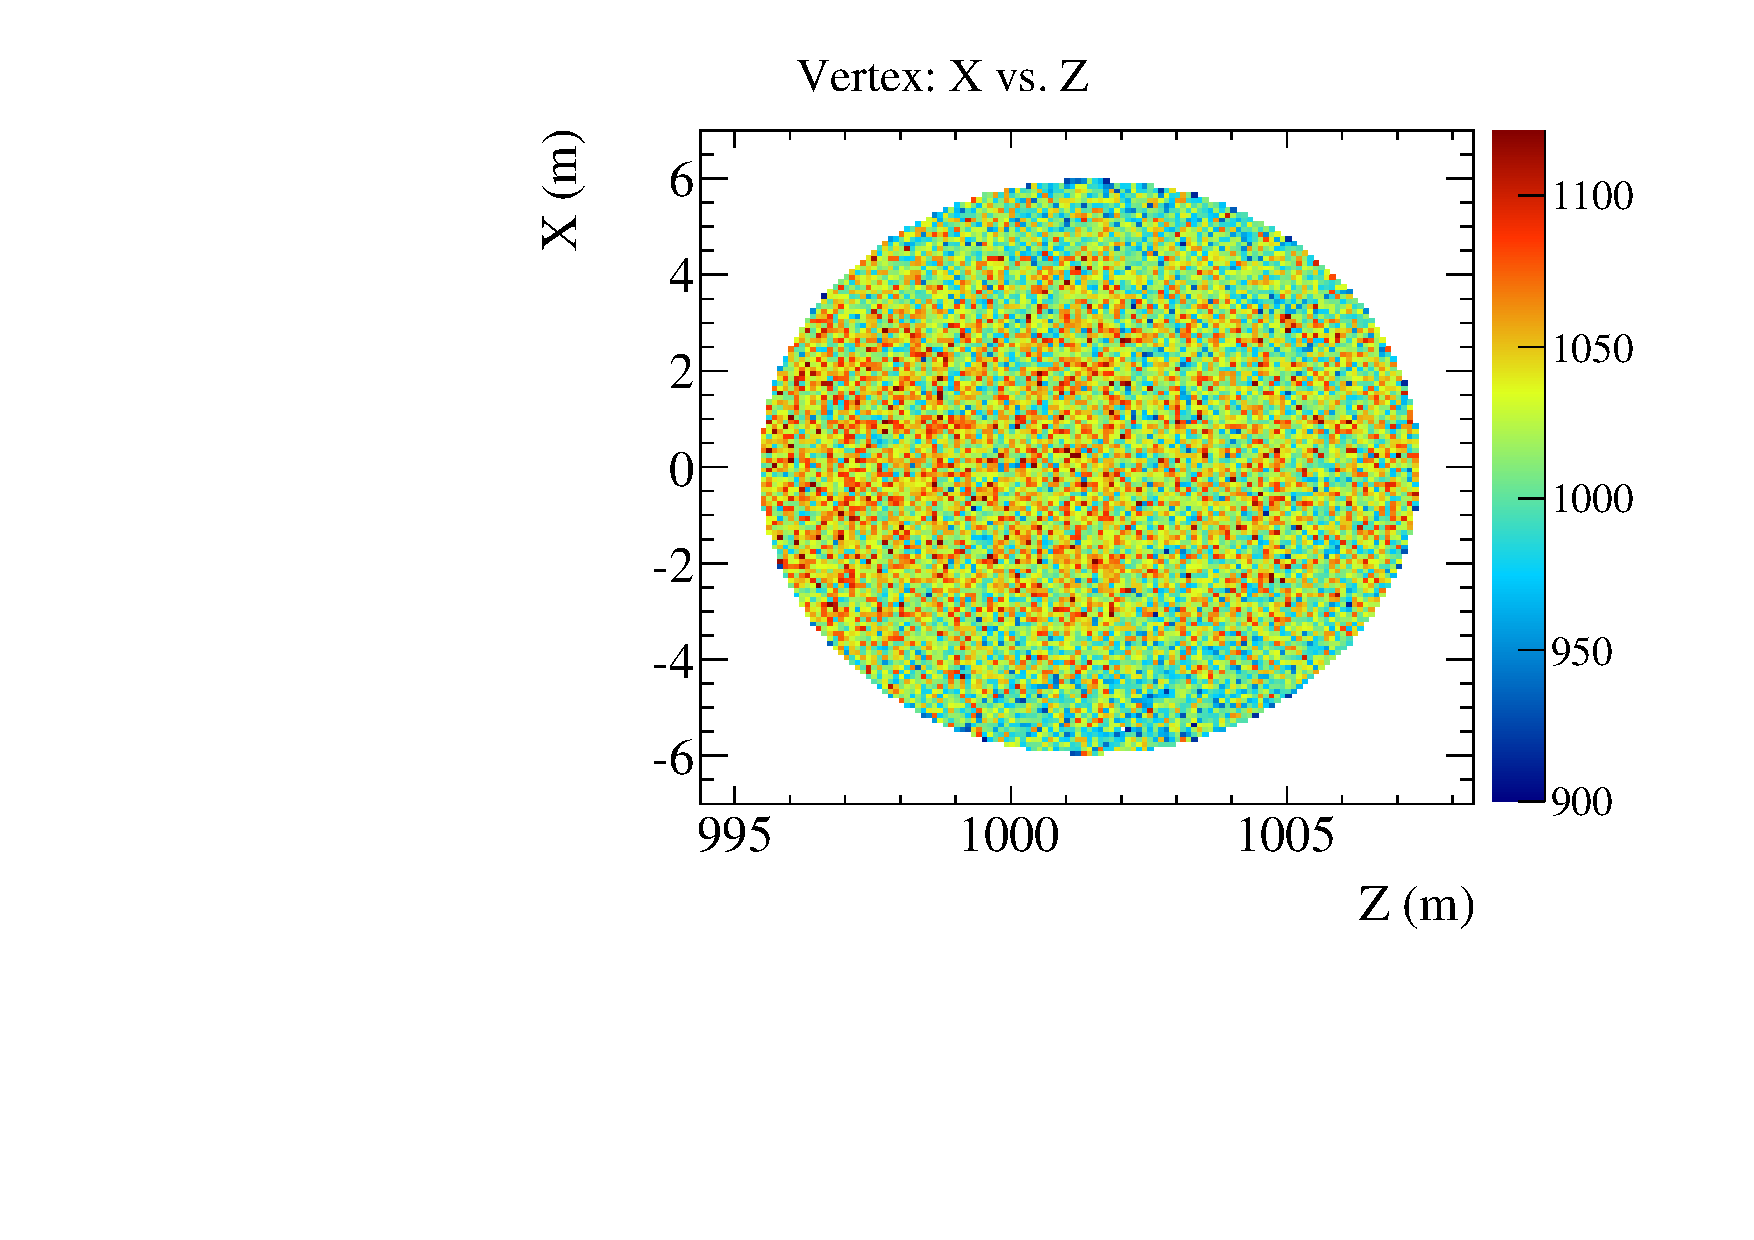
\includegraphics[width=9cm]{figures/vertex_xz.pdf}
    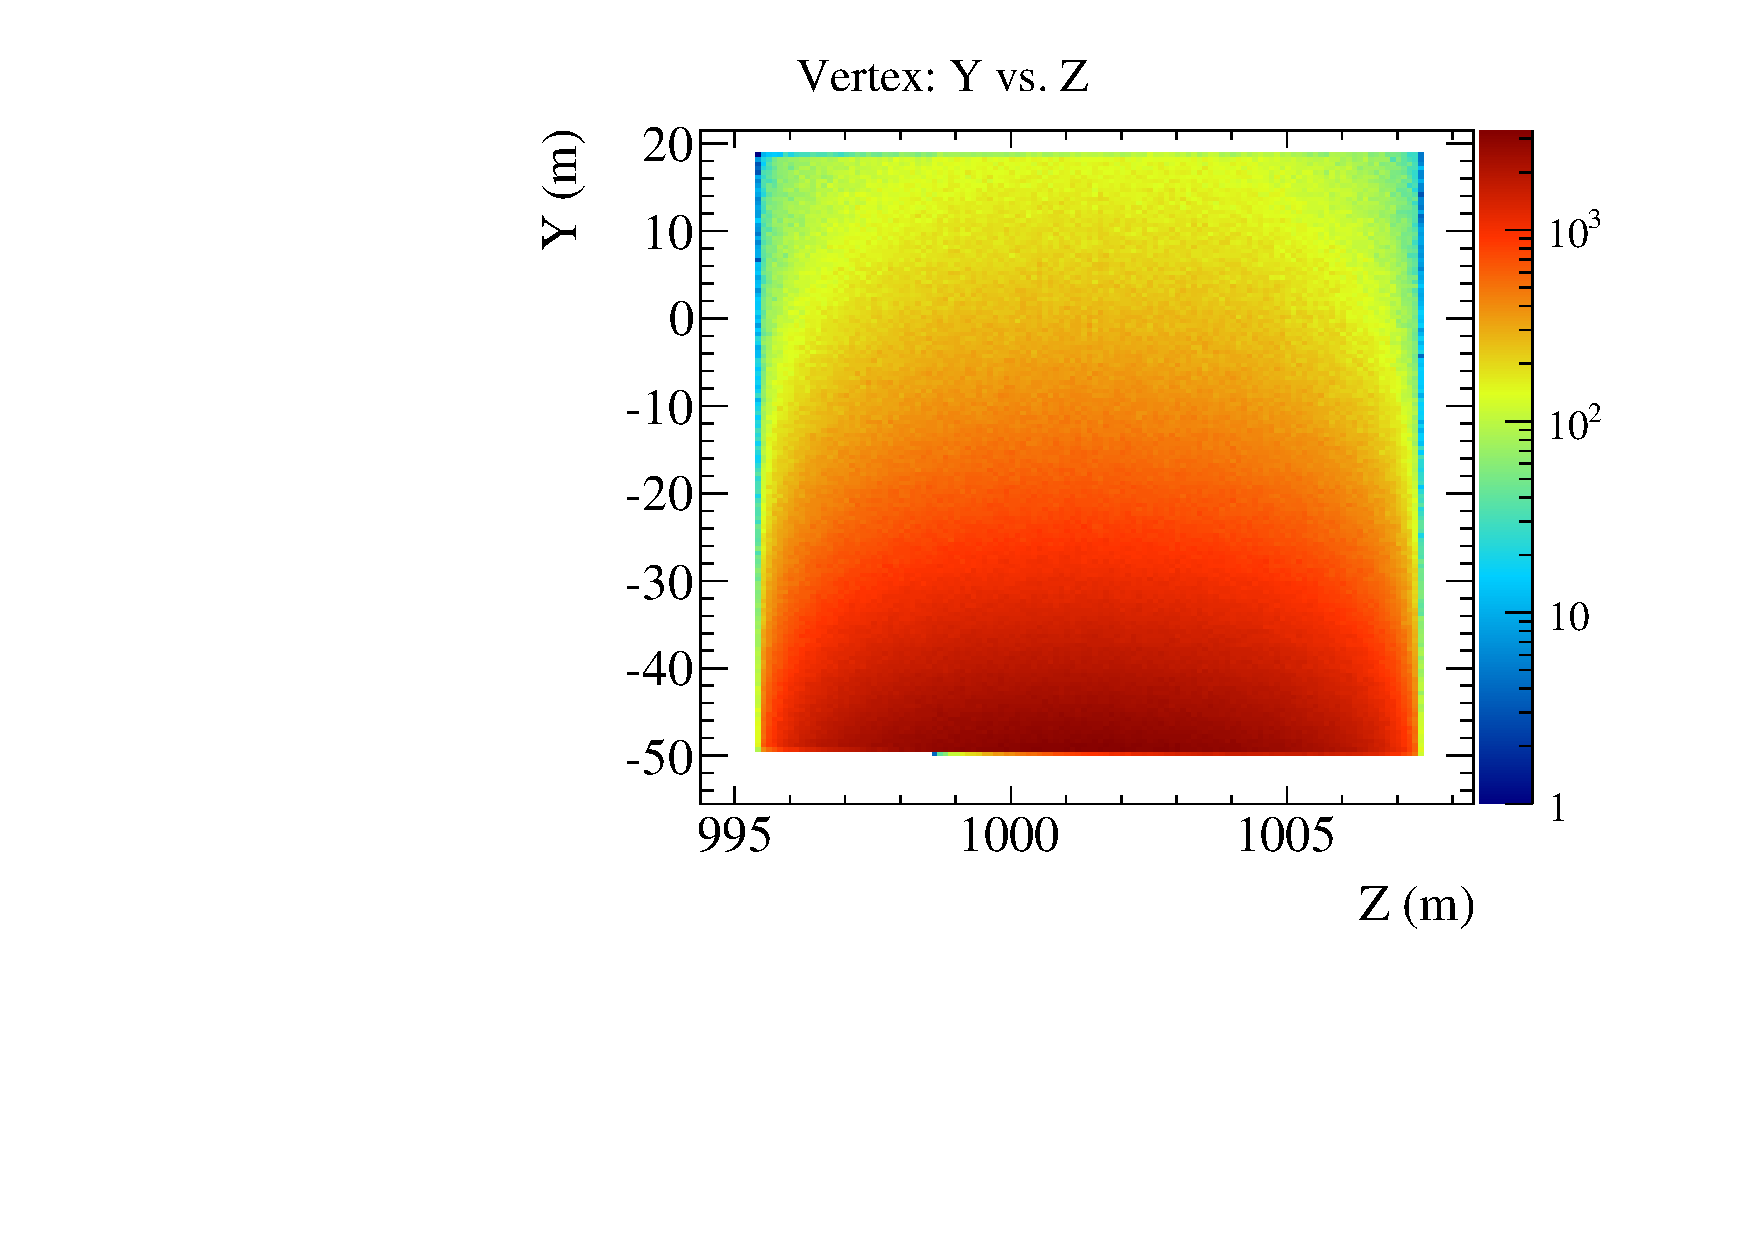
\includegraphics[width=9cm]{figures/vertex_yz.pdf}
    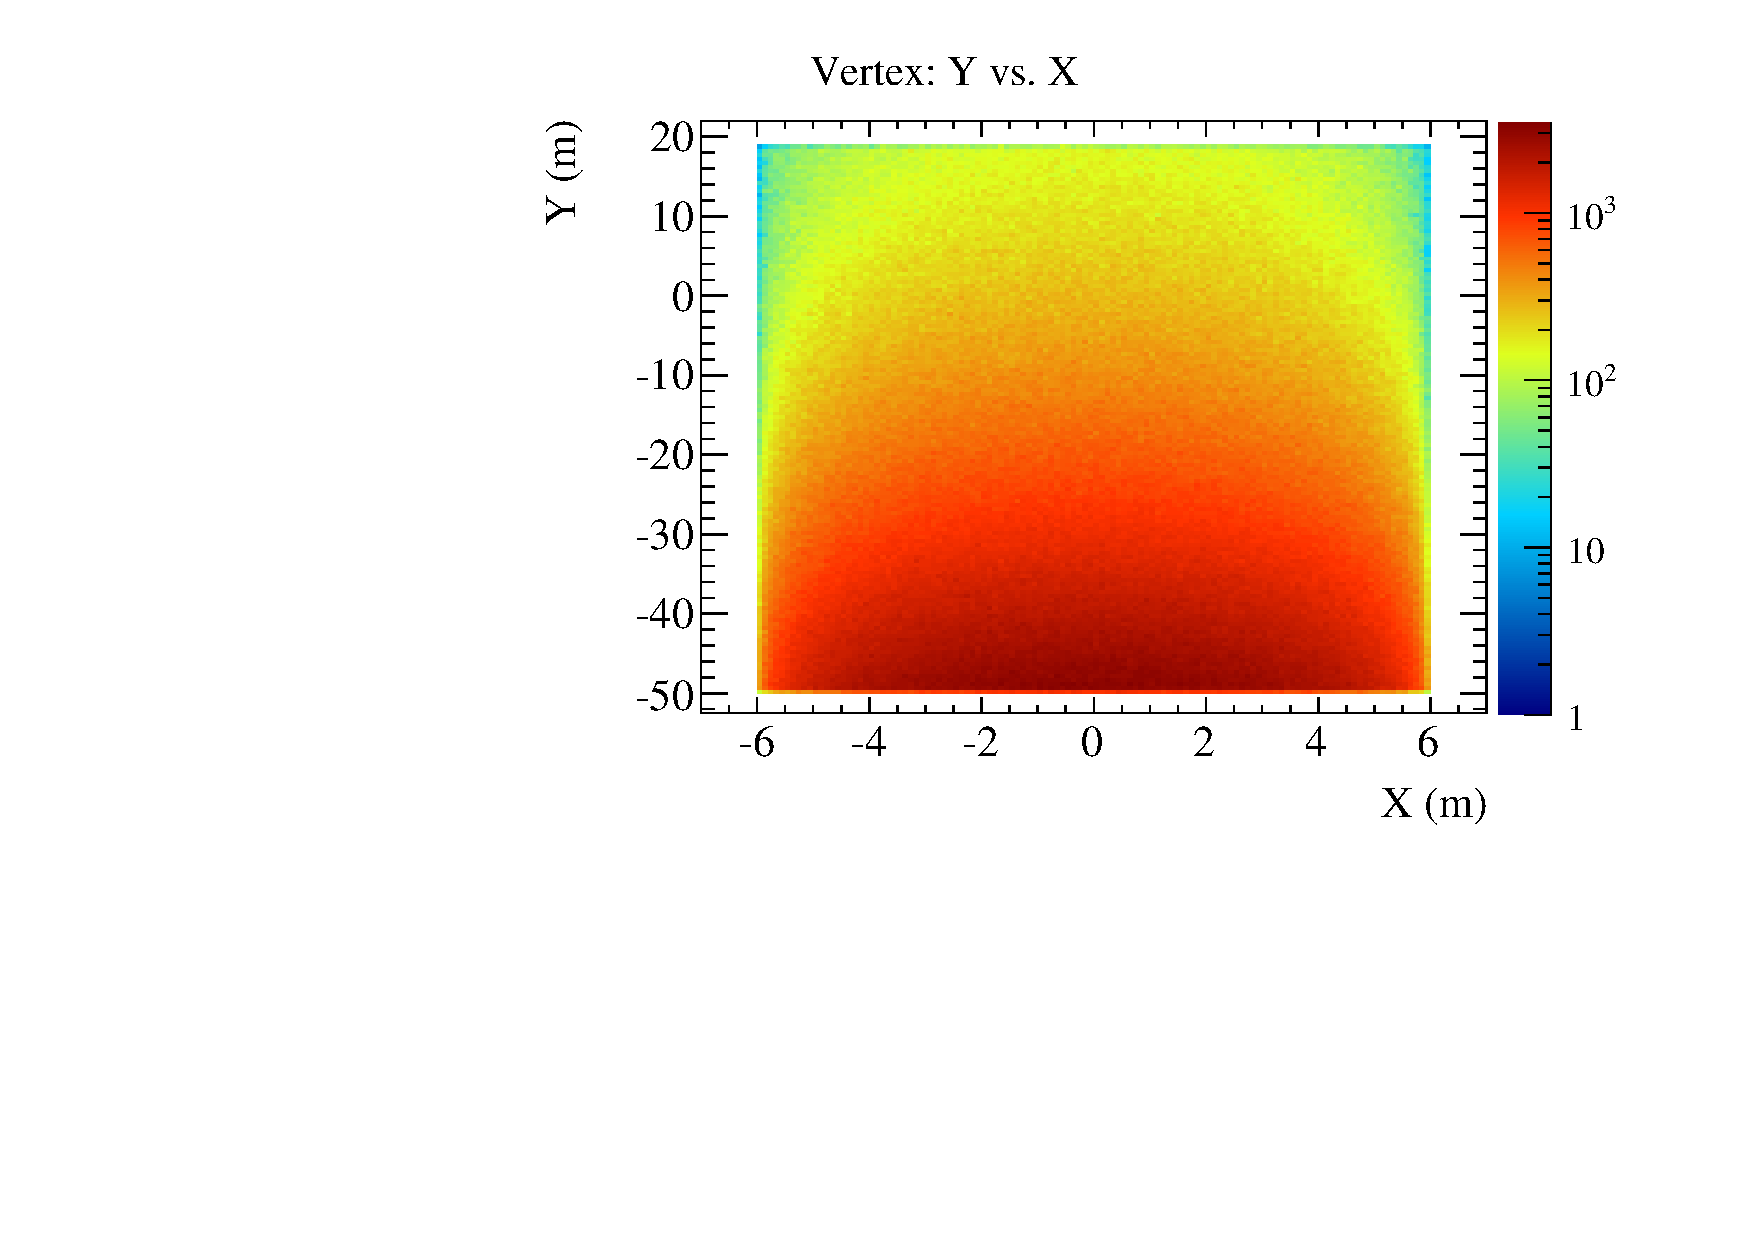
\includegraphics[width=9cm]{figures/vertex_xy.pdf}
    \caption{The distribution of simulated vertices shown in projections to the x-z (top), y-z (middle) and x-y (bottom) planes.  Here
    x is defined as the horizontal axis perpendicular to the beam, z is the horizontal axis in the beam direction and y is the vertical axis. }
    \label{fig:nu_vertex}
  \end{center}
\end {figure}  

%A full detector simulation for \nuprism is not yet ready, so we model the efficiency and resolution for the detection of 
%single electron or muon rings using the known performance of the SK detector and the new reconstruction software developed for T2K, called fiTQun.  Using the SK Monte Carlo,
%efficiency tables are generated for each true event topology, and these tables are binned by the true quantities: distance to the wall of the most energetic particle, $ToWall$; the visible energy of the most energetic particle, $E_{vis}$; and the true neutrino energy, $E_{true}$.  Smearing of the reconstruced $E_{vis}$, ring direction and vertex are also applied.  The resolution histograms are constructed from the SK Monte Carlo for muon and electron ring hypotheses separately and evaluated for bins in true $ToWall$ and $E_{vis}$. 
%
%For each neutrino interaction generated for \nuprism, the true topology, most energetic ring, $E_{vis}$ and $ToWall$ are evaluated.  Then the
%corresponding efficiencies is found from the SK/fiTQun tables and random rejection is applied according to the efficiency.  If the event passes the efficiency step, the resolution histograms are found and the observed quantities are evaluated by smearing the true quantities.

